%%%%%%%%%%%%%%%%%%%%%%%%%%%%%%%%%%%%%%%%%%%%%%%%%%%%%%%%
% Este é um documento que servirá de modelo para
% os relatórios feitos na disciplina Laboratório de Circuitos Lógicos
% 2020-2
%%%%%%%%%%%%%%%%%%%%%%%%%%%%%%%%%%%%%%%%%%%%%%%%%%%%%%%%%

%%%%%%%%%%%%%%%%%%%%%%%%%%%%%%%%%%%%%%%%%%%%%%%%%%%%%%%%%
% Use os diferentes diretórios para colocar os relatórios de cada experimento, deste modo vc consegue manter um histórico e todo material organizado em apenas um local.
% Lembre-se de mudar o Main Document no Menu!!!

\documentclass[12pt]{article}

\usepackage{sbc-template}
\usepackage[brazil]{babel}
\usepackage{graphicx}
\usepackage{url}
\usepackage{float}
\usepackage{listings}
\usepackage{color}
%\usepackage{todonotes}
\usepackage{algorithmic}
\usepackage{algorithm}
\usepackage{hyperref}
\hypersetup{
    colorlinks=true,
    linkcolor=black,
    filecolor=magenta,      
    urlcolor=blue,
    citecolor=black
    }
     
\sloppy

\title{Experimento 5\\ 
Implementação de Circuitos Combinacionais com Multiplexadores}

\author{Grupo B2 - Turma T2\\   
        Allan Victor Almeida Faria, 261010546\\
        Caio César Gonçalves Ribeiro,  211038217\\
        Danilo Alves Ribeiro,  242003754\\
}


\address{Dep. Ciência da Computação -- Universidade de Brasília (UnB)\\
  CIC0231 - Laboratório de Circuitos Lógicos\\
  \today
  \email{allanvictor.almeida@gmail.com, caiocesar20032003@gmail.com, daniloalvesjob@gmail.com}
}

\begin{document} 
\maketitle


\selectlanguage{american}
\begin{abstract}
This report presents the design, synthesis and implementation on an FPGA of three combinational logic circuits described in a hardware description language (HDL): a full adder built from two 8-input multiplexers, a full adder built only from basic logic gates, and a special logic function built from a demultiplexer and a multiplexer. The circuits were synthesized in Quartus-II and recorded on the DE2-70 development kit. Functional and timing simulations, together with tests on the board that went through every input combination, matched the expected truth tables, which validated all three implementations.
\end{abstract}
\selectlanguage{brazil}

\begin{resumo}
Este relatório apresenta o projeto, a síntese e a implementação em FPGA de três circuitos lógicos combinacionais descritos em linguagem de descrição de hardware (HDL): um somador completo construído com dois multiplexadores de 8 entradas, um somador completo construído apenas com portas lógicas básicas e uma função lógica especial construída a partir de um demultiplexador e de um multiplexador. Os circuitos foram sintetizados no Quartus-II e gravados no kit de desenvolvimento DE2-70. As simulações funcional e temporal, junto com os testes na placa percorrendo todas as combinações de entrada, concordaram com as tabelas-verdade esperadas, validando as três implementações.
\end{resumo}



\section{Introdução}
\label{sec:Introducao}

Circuitos digitais combinacionais são aqueles cujas saídas dependem apenas da combinação atual das entradas, e podem ser descritos por tabelas-verdade e expressões booleanas \cite{wakerly90}. Blocos como somadores, multiplexadores e demultiplexadores são a base de sistemas digitais mais complexos, como unidades aritméticas e circuitos de roteamento de dados.

Linguagens de descrição de hardware (HDL) permitem descrever esses circuitos de forma textual, simulá-los e sintetizá-los em dispositivos reconfiguráveis, como os FPGAs. Esse fluxo de projeto torna possível verificar o comportamento do circuito antes de gravá-lo e, depois, confirmá-lo na própria placa.

Neste experimento, foram implementados três circuitos: um somador completo construído com multiplexadores, um somador completo construído com portas lógicas tradicionais e uma função lógica especial construída com um demultiplexador e um multiplexador. Cada circuito foi validado por simulações funcional e temporal e por gravação no FPGA, percorrendo todas as combinações de entrada para comparar as saídas com as tabelas-verdade.



\subsection{Objetivos}
\label{sec:Objetivos}

Projetar circuitos em linguagem de descrição de Hardware, sintetizando-os
e implementando-os em FPGA.

\subsection{Materiais} 
\label{sec:Materiais}
Neste experimento foram utilizados os seguintes materiais e equipamentos:
\begin{itemize}
    \item Software Quartus-II versão 13.0 SP1

    \item Kit de desenvolvimento em FPGA DE2-70 Intel
    
\end{itemize}

\section{Procedimentos e Resultados}
\label{sec:Procedimentos}

Foram sintetizadas três funções lógicas a partir de código HDL
para o DE2-70. Nesse contexto, gravou-se os testes iterando
por cada combinação lógica, de modo a comprovar a corretude
da implementação mediante comparação com a tabela-verdade
das funções.

\subsection{Somador com Multiplexador}
\label{sec:Mux}

A tabela verdade da saída normal e da saída carry de um somador completo são, respectivamente:


\begin{figure}[H]
    \centering
    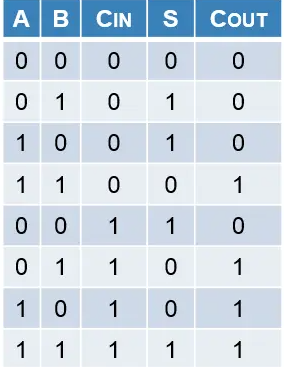
\includegraphics[width=.5\textwidth]{tabelasomador.png}
    \caption{Somador Completo}
    \label{fig:q1}
\end{figure}



Dessa forma, para construção de um somador a partir de dois multiplexadores de 8 entradas, um para
cada saída,
tomaremos A,B, Cin como bits de seleção, e fixaremos as entradas com os valores correspondentes
aos valores esperados para um somador. Por exemplo, ao somarmos 1+1+1, esperamos que ambas 
as saídas estejam em 1. Como isso equivale a selecionar a sétima entrada em cada multiplexador,
fixaremos 1 nessa respectiva entrada. Dessa forma, os códigos em HDL são:



\begin{figure}[H]
    \centering
    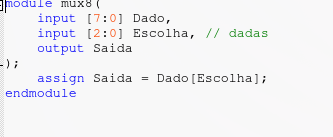
\includegraphics[width=.5\textwidth]{mux8.png}
    \caption{Mux8}
    \label{fig:q2}
\end{figure}



\begin{figure}[H]
    \centering
    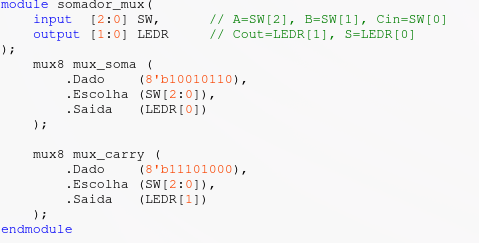
\includegraphics[width=.5\textwidth]{summuxhdl.png}
    \caption{Somador com Multiplexador}
    \label{fig:q3}
\end{figure}


As simulações funcional e temporal mostraram a corretude de nosso modelo. Mais ainda, pode 
se ver a implementação no FPGA nesse \href{https://drive.google.com/file/d/1dFoEPFyvkyebN_j2qbqQsv9ghaUFfVyX/view?usp=drive_link}{link}.:


\begin{figure}[H]
    \centering
    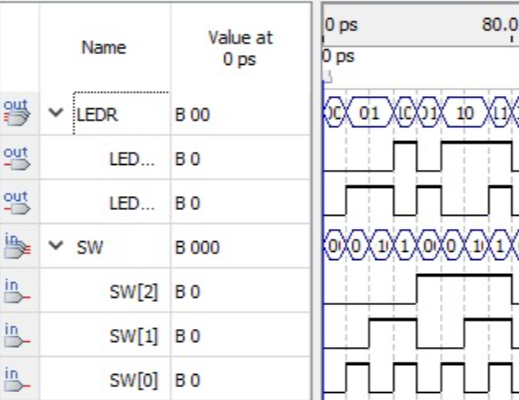
\includegraphics[width=.5\textwidth]{summuxfunc.png}
    \caption{Simulação Funcional do Somador Com Mux}
    \label{fig:q4}
\end{figure}


\begin{figure}[H]
    \centering
    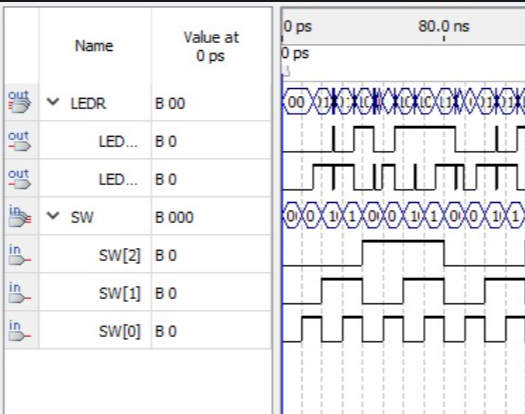
\includegraphics[width=.5\textwidth]{summuxtemp.png}
    \caption{Simulação temporal do somador com Mux}
    \label{fig:q5}
\end{figure}



\subsection{Somador Normal}
\label{sec:Demux}

Implementa-se um somador completo de forma "nativa", usando somente portas lógicas tradicionais.
A lógica se dá da seguinte forma: Para que a saída de carry seja '1', basta que duas das entradas
sejam '1'. Já para que a saída comum seja '1', o número de '1's nas entradas deve ser ímpar, o que
é representado pela função XOR\cite{wakerly90}. O código então é:

\begin{figure}[H]
    \centering
    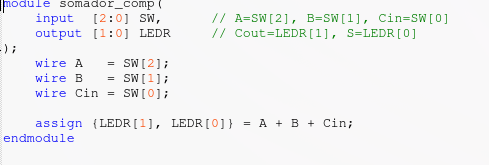
\includegraphics[width=.5\textwidth]{somadorhdl.png}
    \caption{Còdigo do Somador Completo}
    \label{fig:q6}
\end{figure}

O circuito foi sintetizado no FPGA, o que pode ser conferido nesse \href{https://drive.google.com/file/d/1N62ObaMJhtwip5XoDJ2DXeVjFkb4ecKe/view?usp=drive_link}{link}.
Também foram feitas as simulações, que mostraram resultado idêntico ao outro somador:

\begin{figure}[H]
    \centering
    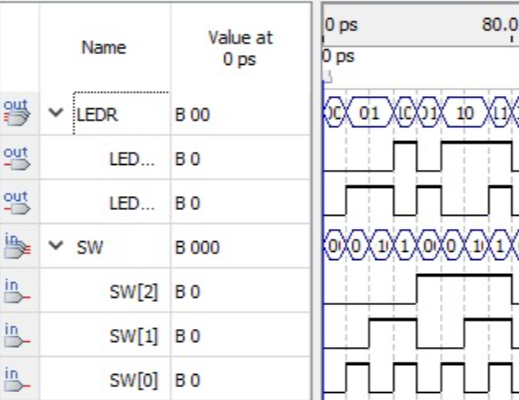
\includegraphics[width=.5\textwidth]{summuxfunc.png}
    \caption{Simulação funcional do Somador}
    \label{fig:q7}
\end{figure}

\begin{figure}[H]
    \centering
    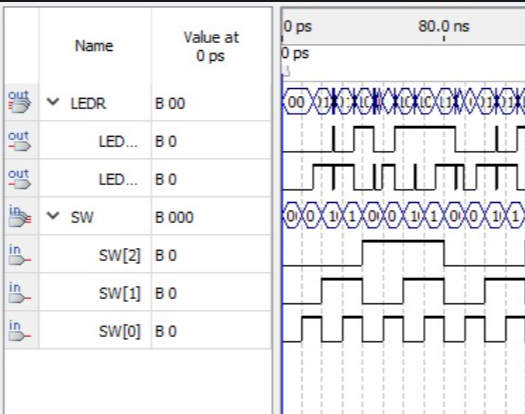
\includegraphics[width=.5\textwidth]{summuxtemp.png}
    \caption{Simulação Temporal do Somador}
    \label{fig:q8}
\end{figure}

\subsection{Função Especial}

Foi construída, a partir de um demultiplexador e do multiplexador, uma função lógica.
O código HDL da função e do multiplexador é dado por:

\begin{figure}[H]
    \centering
    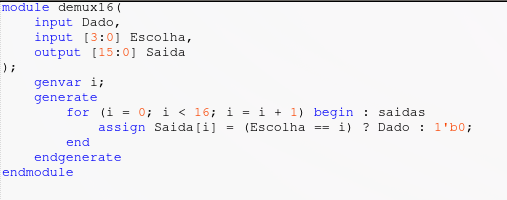
\includegraphics[width=.5\textwidth]{demuxhdl.png}
    \caption{Código do Demultiplexador}
    \label{fig:q9}
\end{figure}

\begin{figure}[H]
    \centering
    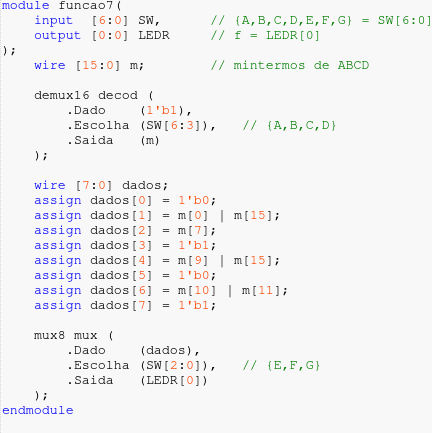
\includegraphics[width=.5\textwidth]{funcao7hdl.png}
    \caption{Código da Função}
    \label{fig:q10}
\end{figure}

Observou-se, tanto nas simulações, quanto no circuito sintetizado
(cuja gravação pode ser vista \href{https://drive.google.com/file/d/19dGameKy70aLvt4kIDSw6L9Ls2EbMcVs/view?usp=drive_link}{aqui})
a corretude do modelo, que respondeu '1' nos mintermos esperados. Atenta-se para a peridiocidade dos mintermos com FG, o termo 
mais abrangente da função:

\begin{figure}[H]
    \centering
    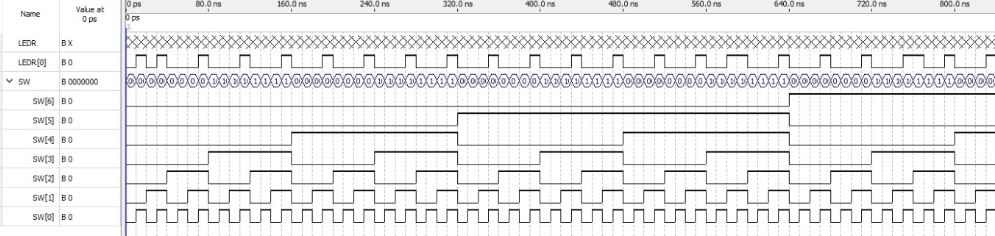
\includegraphics[width=.75\textwidth]{sumfuncfunc.png}
    \caption{Simulação Funcional da Função}
    \label{fig:q11}
\end{figure}

\begin{figure}[H]
    \centering
    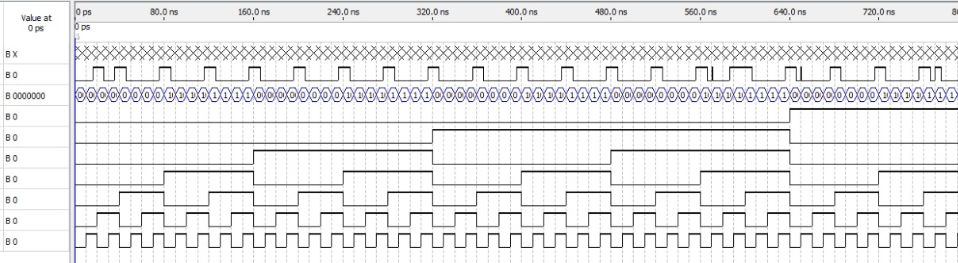
\includegraphics[width=.75\textwidth]{sumfunctemp.png}
    \caption{Simulação Temporal da Função}
    \label{fig:q12}
\end{figure}


\section{Conclusões}

Os três circuitos projetados foram descritos em HDL, sintetizados e gravados com sucesso no FPGA DE2-70. Em todos os casos, as simulações funcional e temporal e os testes na placa, percorrendo todas as combinações de entrada, concordaram com as tabelas-verdade esperadas, o que comprova a corretude das implementações.

O somador com multiplexadores e o somador com portas lógicas apresentaram resultados idênticos, mostrando que uma mesma função pode ser implementada por estruturas diferentes. Já a função especial respondeu '1' exatamente nos mintermos esperados, incluindo a periodicidade associada ao termo FG.

Assim, o objetivo do experimento foi atingido: projetar circuitos em HDL, sintetizá-los e implementá-los em FPGA.
\label{sec:Conclusao}

 


\bibliographystyle{plain}
\bibliography{relatorio}  %Aqui é a definição do arquivo .bib a ser usado pelas referências


\newpage 
% Colocar aqui apenas as respostas dos itens da Auto-Avaliação
\section*{Auto-Avaliação}

\begin{enumerate}
    \item v
    \item v 
    \item f 
    \item v 
    \item v 
    \item v 
    \item v 
    \item f 
    \item v 
    \item f 
    \item v
\end{enumerate}


\end{document}
